\chapter{Test}
Dette kapitel vil indeholde en kort beskrivelse af de tests som er blevet udført i forhold til validering af Rambøll Tilsyn. \\
For den fulde test dokumentation, henvises til Modul- og Integrationstest dokumentet i bilag. \\

\section{Automatiseret test}
I følgende afsnit beskrives unit test der er lavet. Framworket Nunit\cite{NUnit} er blevet brugt til vores testing af klasser. 

\textbf{Validator}
Validator-klassen er en statisk klasse, som har håndterer validering af input felterne i applikationen. Applikationens testcases kan ses på Figur \ref{fig:ValidatorUnit}.
\begin{figure}[H]
	\centering
	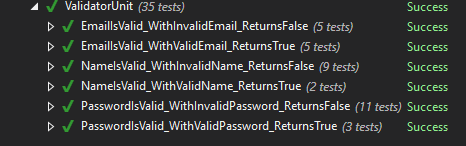
\includegraphics[width=0.6\linewidth]{Test/ValidatorUnit}
	\caption{Screenshot af test sessionen på ValidatorUnit}
	\label{fig:ValidatorUnit}
\end{figure}

\section{Manuel test}
I følgende afsnit beskrives de manuelle test cases for 'Login' viewet til Rambøll Tilsyn.

\textbf{Login tests} \\
Denne sektion indeholder de manuelle tests for 'Login' viewet. Der er skrevet tilsvarende test cases for alle de implementerede views. Disse kan findes i Modul- og Integrationstest dokumentets afsnit \ref{Test-sec:ManuelTest}. \\ \\
\textbf{Pass/fail criteria:} \\
Alle steps skal verificeres på Rambøll Tilsyn applikationen:
\begin{itemize}[-]
	\item Verificer at bruger kan logge ind med korrekte brugeroplysninger.
	\item Verificer at bruger ikke kan logge ind med forkert email.
	\item Verificer at bruger ikke kan logge ind med forkert kodeord.
\end{itemize}
De manuelle tests til Rambøll Tilsyn, er med til at sikre både funktionalitet og flow i applikationen fungerer.